\section{Energy Calculations}\label{sc:energyCalculations}
%TODO add section reference for energy lab
In every wireless network system energy consumption is a must to evaluate. Based on measurement, see section ???, some calculations were made. Since power consumption is not the main investigation of the project, only lifetime for the base station is done in theory. An assumption of every package is send directly to the sink successfully and immediately a respond is send also successfully. Total latency between the two nodes is set as constant to 12 milliseconds and an overshoot time at powerup from sleep mode is also constant at 50 milliseconds and $40\%$ extra energy related to receiving energy. Overshoot after wakeup is modelled as a gaussian function as shown in Figure \ref{fig:gaussianDistributionsOfVoltagePeak} for max energy wakeup. Table 1 shows the lifetime of the base station at six different scenarios all assuming two full AA-batteries.%TODO reference to https://en.wikipedia.org/wiki/AA_battery "RAM"
Scenario 1: Full power at transmission and otherwise always listening for packages.
Scenario 2: Min power at transmission and otherwise always listening for packages.
Scenario 3: Full power at transmission, only listening for packages when receiving and no overshoot.
Scenario 4: Min power at transmission, only listening for packages when receiving and no overshoot.
Scenario 5: Full power at transmission, only listening for packages when receiving and overshoot at power up.
Scenario 6: Min power at transmission, only listening for packages when receiving and overshoot at power up.
Calculations are in appendix ?? and even though it cost to power up from sleep mode, it is still gives longer life time to put the nodes to sleep.

%Figure 13
\begin{figure}[H]
	\centering
	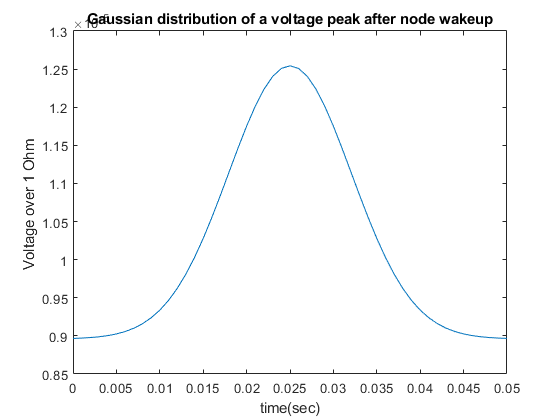
\includegraphics[width=\linewidth]{theory/energyCalculations/fig/gaussianDistributionsOfVoltagePeak.png}
	\caption{Start up voltage peak after sleep mode.}
	\label{fig:gaussianDistributionsOfVoltagePeak}
\end{figure}
